% EclipseFP-JE.tex
\begin{hcarentry}[updated]{EclipseFP}
\report{JP Moresmau}%11/12
\status{stable, maintained, and actively developed}
\participants{building on code from B.\ Scott Michel, Alejandro Serrano, Thiago Arrais, Leif Frenzel, Thomas ten Cate, Martijn Schrage, Adam Foltzer and others}
\makeheader

%**<img width=500 src="./eclipsefp-screenshot1.jpg">
%*ignore
\begin{center}
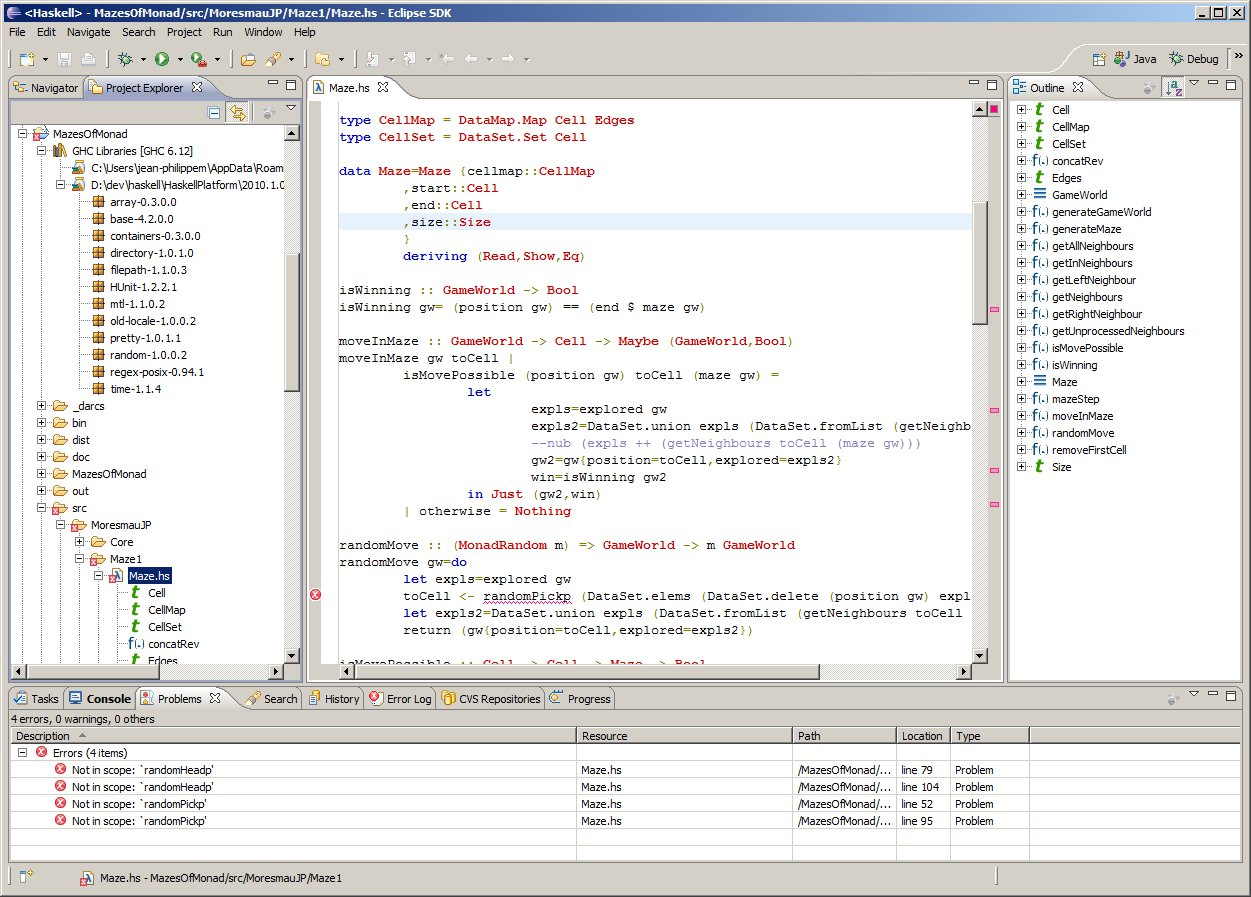
\includegraphics[width=0.47\textwidth]{html/eclipsefp-screenshot1.jpg}
\end{center}
%*endignore

EclipseFP is a set of Eclipse plugins to allow working on Haskell code projects. Its goal is to offer a fully featured Haskell IDE in a platform developers coming from other languages may already be familiar with.
It features Cabal integration (.cabal file editor, uses Cabal settings for compilation, allows the user to install Cabal packages from within the IDE), and GHC integration. Compilation is done via the GHC API, syntax coloring uses the GHC Lexer. Other standard Eclipse features like code outline, folding, and quick fixes for common errors are also provided. HLint suggestions can be applied in one click. EclipseFP also allows launching GHCi sessions on any module including extensive debugging facilities: the management of breakpoints and the evaluation of variables and expressions uses the Eclipse debugging framework, and requires no knowledge of GHCi syntax. It uses the BuildWrapper Haskell tool to bridge between the Java code for Eclipse and the Haskell APIs. It also provides a full package and module browser to navigate the Haskell packages installed on your system, integrated with Hackage.
The source code is fully open source (Eclipse License) on github and anyone can contribute. Current version is 2.3.2, released in October 2012 and supporting GHC 7.0 and above, and more versions with additional features are planned and actively worked on. Feedback on what is needed is welcome! The website has information on downloading binary releases and getting a copy of the source code. Support and bug tracking is handled through Sourceforge forums.

\FurtherReading 
\url{http://eclipsefp.github.com/}
\end{hcarentry}
